\setlength{\columnsep}{1cm}

\begin{multicols}{2}
	Тестируемый демультиплексор 1-в-4 должен соответствовать следующей таблице истинности, где \( Y \) — вход, \( S_1 \) и \( S_2 \) — управляющие сигналы, а \( Z_0 \), \( Z_1 \), \( Z_2 \) и \( Z_3 \) — выходы.

	Временная диаграмма на Рисунке 10 показывает изменение напряжений на входах \( Y \), \( S_1 \), \( S_2 \) и выходах \( Z_0 \), \( Z_1 \), \( Z_2 \), \( Z_3 \) во времени, подтверждая правильность работы демультиплексора.

	\columnbreak

	\noindent
	% \vspace*{0.1cm}
	\renewcommand{\arraystretch}{1.12}
	\raggedright
	\begin{tabular}{|>{\centering\arraybackslash}p{0.8cm}|>{\centering\arraybackslash}p{0.8cm}|>{\centering\arraybackslash}p{0.8cm}|>{\centering\arraybackslash}p{0.8cm}|>{\centering\arraybackslash}p{0.8cm}|>{\centering\arraybackslash}p{0.8cm}|>{\centering\arraybackslash}p{0.8cm}|}
		\hline
		$S_1$ & $S_2$ & $Y$ & $Z_0$ & $Z_1$ & $Z_2$ & $Z_3$ \\
		\hline
		0     & 0     & 1   & 1     & 0     & 0     & 0     \\
		0     & 1     & 1   & 0     & 1     & 0     & 0     \\
		1     & 0     & 1   & 0     & 0     & 1     & 0     \\
		1     & 1     & 1   & 0     & 0     & 0     & 1     \\
		\hline
		0     & 0     & 0   & 0     & 0     & 0     & 0     \\
		0     & 1     & 0   & 0     & 0     & 0     & 0     \\
		1     & 0     & 0   & 0     & 0     & 0     & 0     \\
		1     & 1     & 0   & 0     & 0     & 0     & 0     \\
		\hline
	\end{tabular}

\end{multicols}

\begin{figure}[H]
	\centering
	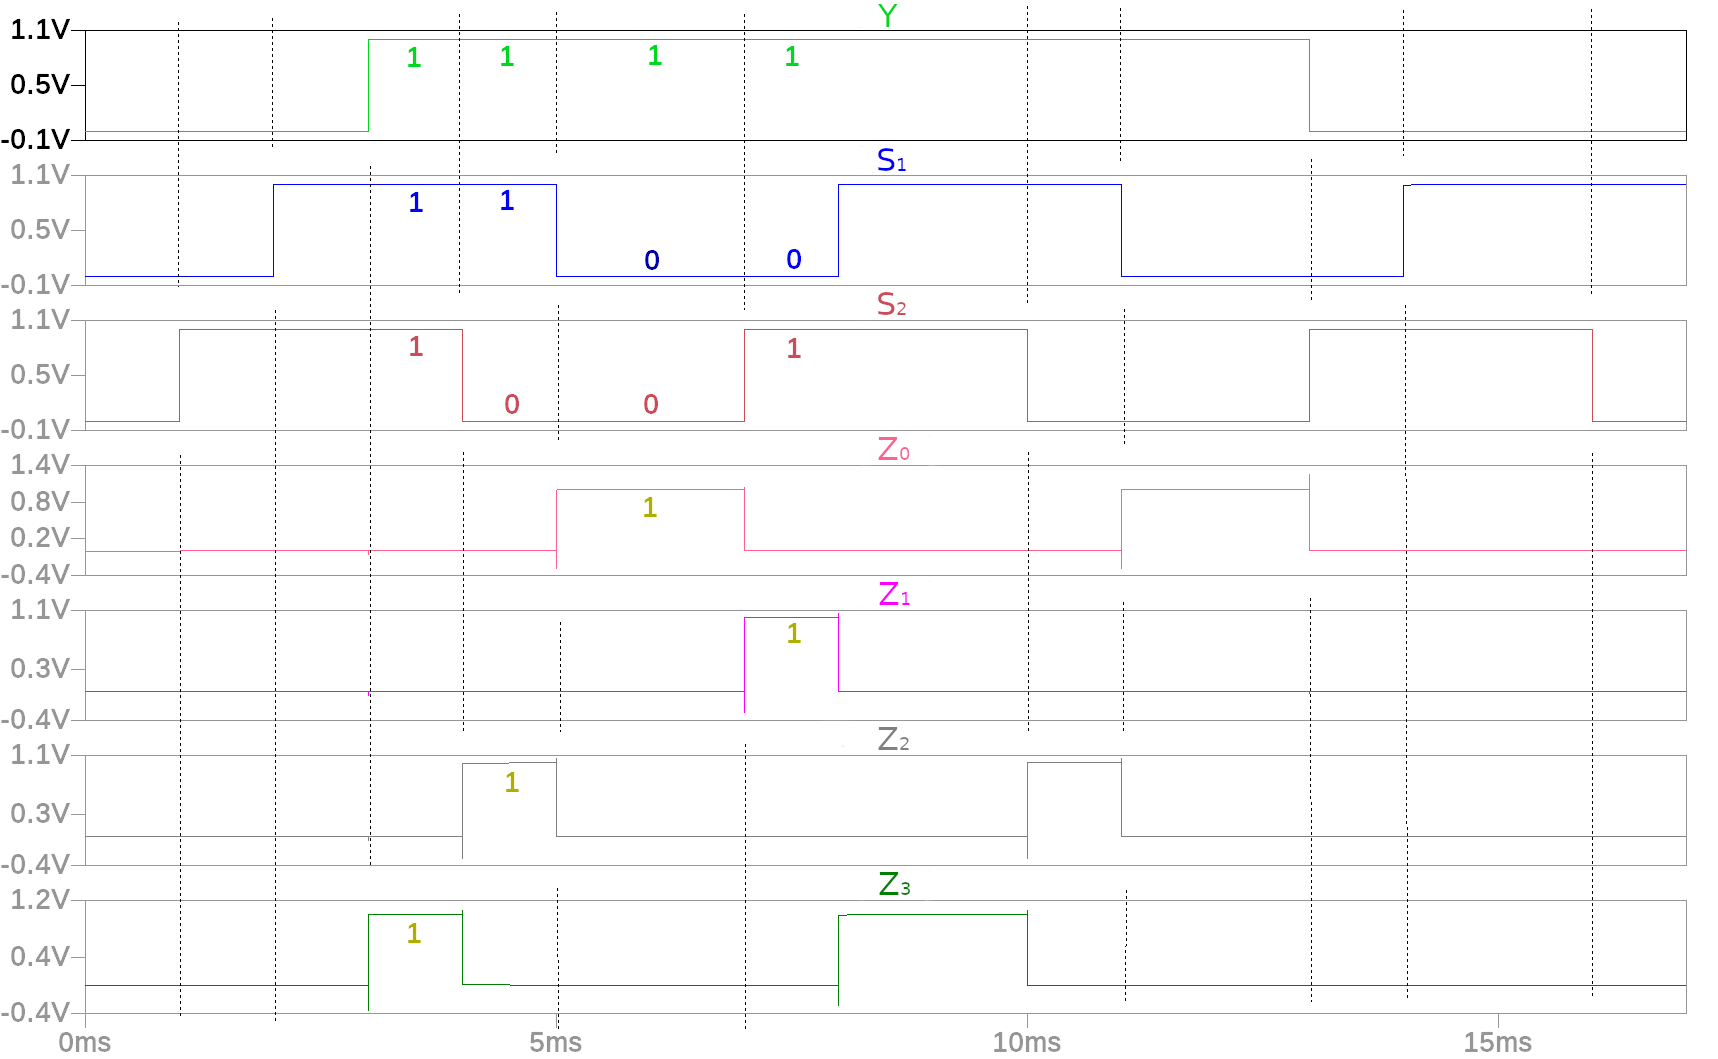
\includegraphics[width=1\textwidth]{../data/test_boe_time}
	\caption{Временная диаграмма напряжений на $Z_0, Z_1, Z_2, Z_3, S_1, S_2, Y$}
\end{figure}
